\documentclass[10pt,ignorenonframetext,x11names, dvipsnames, bibspacing,natbib]{beamer}
\setbeamertemplate{caption}[numbered]
\setbeamertemplate{caption label separator}{: }
\setbeamercolor{caption name}{fg=normal text.fg}
\beamertemplatenavigationsymbolsempty
\usepackage{lmodern}
\usepackage{amssymb,amsmath}
\usepackage{ifxetex,ifluatex}
\usepackage{fixltx2e} % provides \textsubscript
\ifnum 0\ifxetex 1\fi\ifluatex 1\fi=0 % if pdftex
  \usepackage[T1]{fontenc}
  \usepackage[utf8]{inputenc}
\else % if luatex or xelatex
  \ifxetex
    \usepackage{mathspec}
  \else
    \usepackage{fontspec}
  \fi
  \defaultfontfeatures{Ligatures=TeX,Scale=MatchLowercase}
\fi
\usetheme[]{Rafal_beamerSly1}
% use upquote if available, for straight quotes in verbatim environments
\IfFileExists{upquote.sty}{\usepackage{upquote}}{}
% use microtype if available
\IfFileExists{microtype.sty}{%
\usepackage{microtype}
\UseMicrotypeSet[protrusion]{basicmath} % disable protrusion for tt fonts
}{}
\newif\ifbibliography
\hypersetup{
            pdftitle={A bayesian method of cosine-based word2vec bias estimation},
            pdfauthor={Alicja Dobrzeniecka \& Rafal Urbaniak (LoPSE research group, University of Gdansk)},
            colorlinks=true,
            linkcolor=Maroon,
            citecolor=Blue,
            urlcolor=blue,
            breaklinks=true}
\urlstyle{same}  % don't use monospace font for urls

% Prevent slide breaks in the middle of a paragraph:
\widowpenalties 1 10000
\raggedbottom

\AtBeginPart{
  \let\insertpartnumber\relax
  \let\partname\relax
  \frame{\partpage}
}
\AtBeginSection{
  \ifbibliography
  \else
    \let\insertsectionnumber\relax
    \let\sectionname\relax
    \frame{\sectionpage}
  \fi
}
\AtBeginSubsection{
  \let\insertsubsectionnumber\relax
  \let\subsectionname\relax
  \frame{\subsectionpage}
}

\setlength{\parindent}{0pt}
\setlength{\parskip}{6pt plus 2pt minus 1pt}
\setlength{\emergencystretch}{3em}  % prevent overfull lines
\providecommand{\tightlist}{%
  \setlength{\itemsep}{0pt}\setlength{\parskip}{0pt}}
\setcounter{secnumdepth}{0}

\title{\large A bayesian method of cosine-based word2vec bias estimation}
\author{Alicja Dobrzeniecka \& Rafal Urbaniak \footnotesize \newline (LoPSE
research group, University of Gdansk)}
\date{ExpSem2021, ESSLLI}

\begin{document}
\frame{\titlepage}

\begin{frame}

\frametitle{The gist of the project}

\pause

\begin{block}{Classical probabilism in epistemology (and in
applications)}

Represent uncertainty by a single probabilistic measure (point
estimates).

\vspace{-3mm}

\begin{align*}
\pr(\mathsf{recovery}\vert \mathsf{treatment}) & = .6\\
\end{align*}

\vspace{-6mm}

\pause

\end{block}

\begin{block}{Imprecise probabilism}

Evidence (e.g.~expert evidence) sometimes fails to warrant such
precision.

\vspace{-3mm}

\begin{align*}
\pr(\mathsf{recovery}\vert \mathsf{treatment}) & \in [.4,.6]\\
\end{align*}

\vspace{-6mm}

\pause 

\end{block}

\begin{block}{Epistemological difficulties of imprecise probabilism}

\begin{itemize}
\item
  hard to model the weight of and combine evidence.
\item
  inertia of agnosticism.
\item
  growth of uncertainty in light of new evidence.
\end{itemize}

\end{block}

\end{frame}

\begin{frame}{The gist of the project}

\begin{block}{My novel contribution}

\begin{itemize}
\item
  Meet the desiderata motivating imprecision.
\item
  Avoid these difficulties.
\item
  Do so by using higher-order probabilities.
\end{itemize}

\begin{center}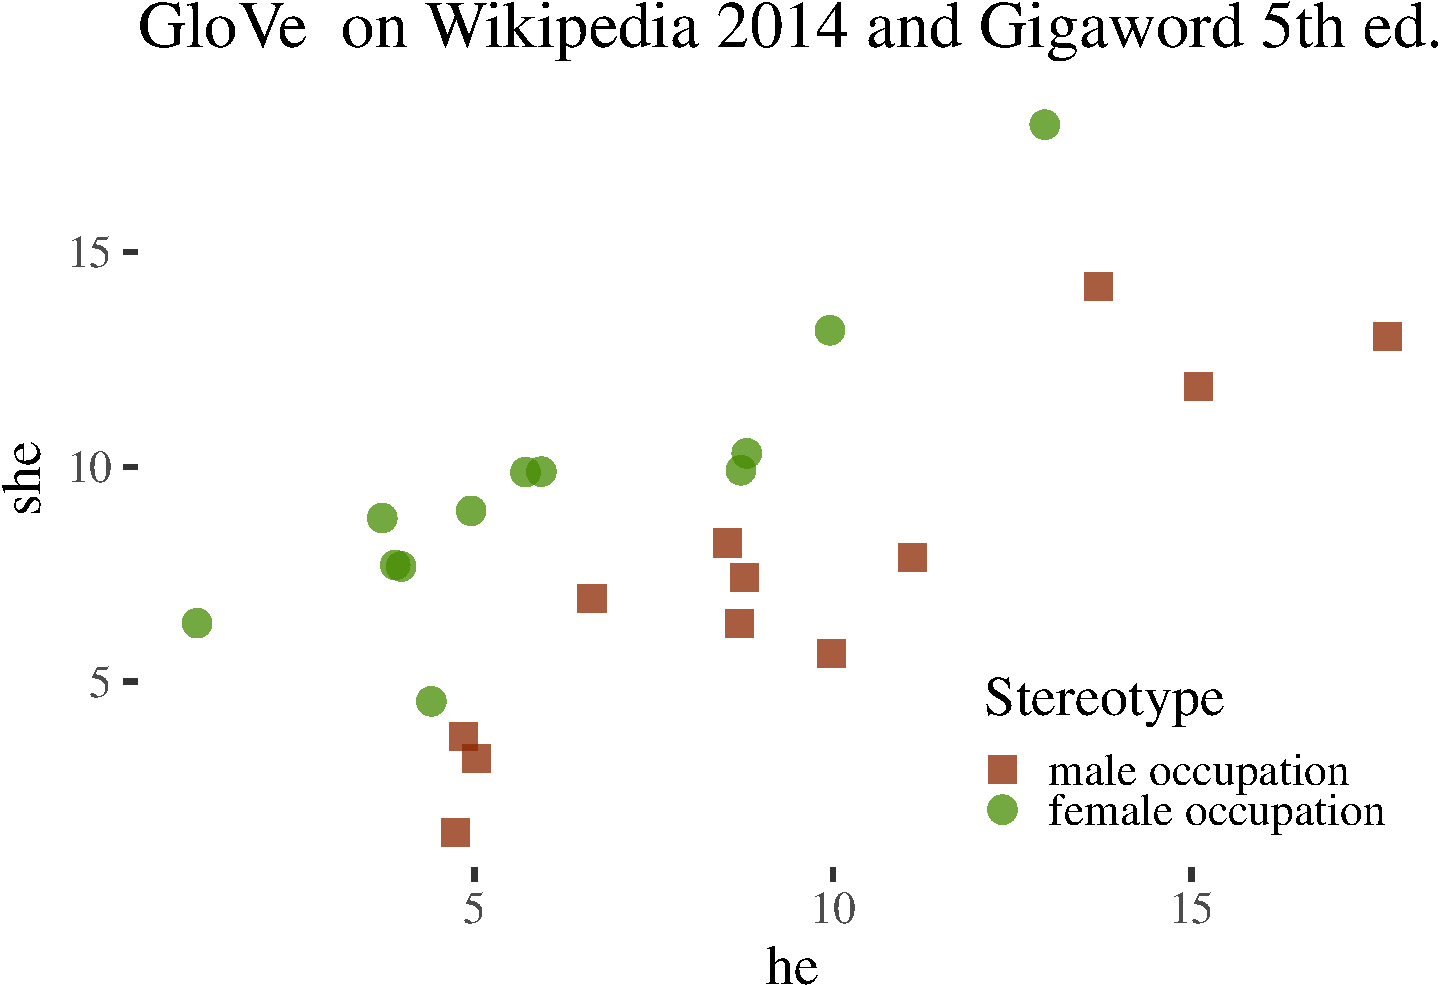
\includegraphics[width=0.7\linewidth]{presentationESSLLI_files/figure-beamer/unnamed-chunk-1-1} \end{center}

\end{block}

\end{frame}

\begin{frame}{Motivations for imprecision \large (straighforward
considerations)}

\pause

\begin{block}{Radical lack of information}

\(\pr(\mathsf{It \,\, will \,\, snow\,\, in\,\, Boston\,\, on \,\, New\,\, Year's\,\, Eve\,\, 2026}) =\)
?

\pause

\end{block}

\begin{block}{Weight of evidence}

\begin{itemize}
\tightlist
\item
  You've seen 4/10 patients recover. \(\pr(\mathsf{recovery})=.4\)?
\end{itemize}

\pause
\vspace{-2mm}

\begin{itemize}
\tightlist
\item
  You've seen 40/100 patients recover. \(\pr(\mathsf{recovery})=.4\)?
\end{itemize}

\footnotesize (You could try to use classical statistical tools, such as
confidence intervals,\linebreak  but they have their own problems.)

\end{block}

\end{frame}

\begin{frame}{Motivations for imprecision \large (uniformity and
agnosticism)}

\begin{block}{Agnosticism preservation requirement}

Agnosticism about uniquely connected variables should be the same.

\vspace{-5mm}

\[X \mbox{ and } Y=X+2 \mbox{ or } Z = X^2 \,\,\, \mbox{ for $10>X>0$.}\]

\pause

\end{block}

\begin{block}{The trouble}

\begin{center}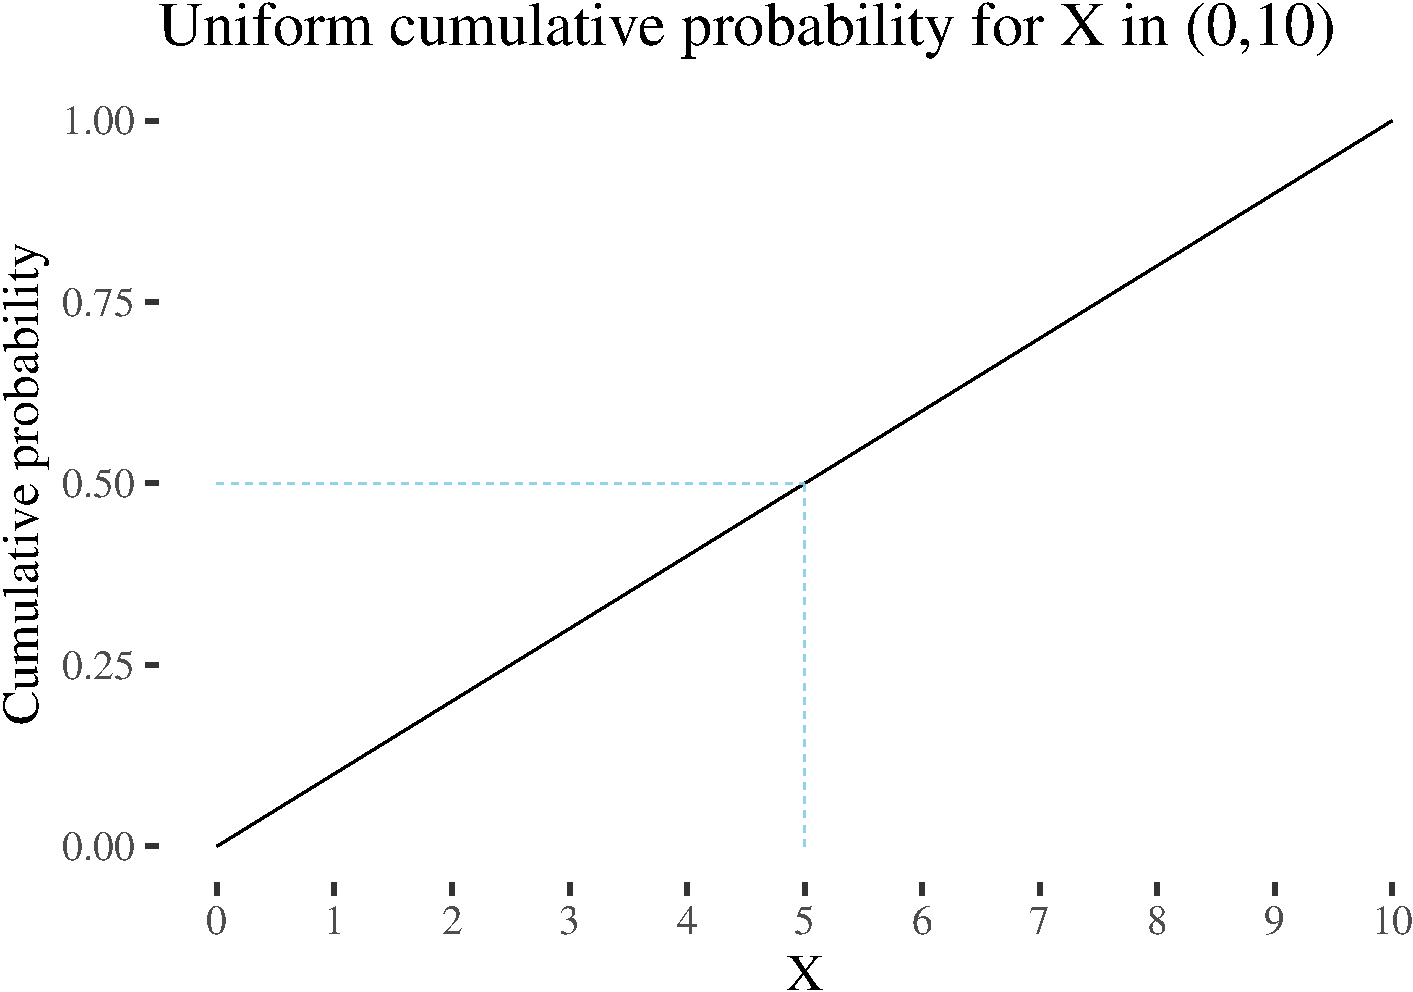
\includegraphics[width=0.6\linewidth]{presentationESSLLI_files/figure-beamer/unnamed-chunk-2-1} \end{center}

\vspace{-9mm}

\begin{align*}\pr(X<5) = .5 = \pr(X^2 < 25)
\end{align*}

\end{block}

\end{frame}

\begin{frame}{Motivations for imprecision \large (uniformity and
agnosticism)}

\begin{block}{The trouble}

\begin{center}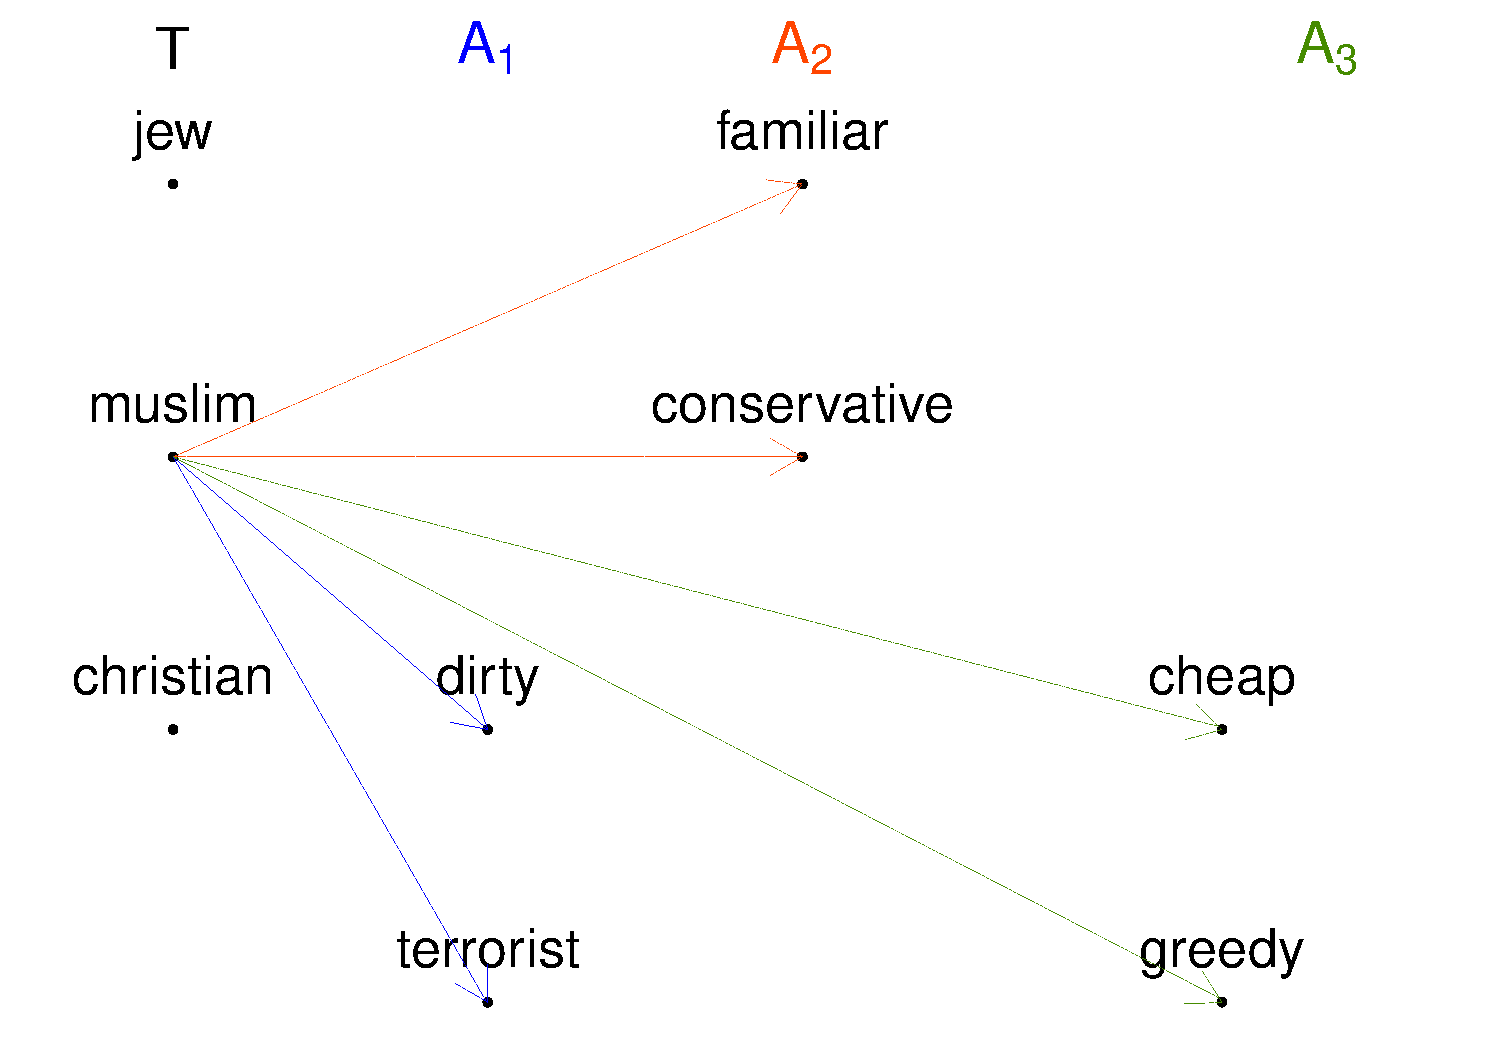
\includegraphics[width=0.6\linewidth]{presentationESSLLI_files/figure-beamer/unnamed-chunk-3-1} \end{center}

\end{block}

\end{frame}

\begin{frame}{Motivations for imprecision \large (expert evidence)}

\begin{block}{Weather forecasters}

\vspace{-1mm}

\begin{tabular}{ll}
Al: & $\pr(\mathsf{It \,\,  will\,\,  rain\,\,  tomorrow})=.6$\\
Bert: & $\pr(\mathsf{It \,\,  will\,\,  rain\,\,  tomorrow})=.8$
\end{tabular}

\pause

\end{block}

\begin{block}{Linear pooling}

\vspace{-4mm}

\begin{align*}
\pr(\mathsf{It \,\,  will\,\,  rain\,\,  tomorrow}) & = 
\alpha \times .6 + \beta \times .8 \,\,\,\,\,  (where \,\, \alpha + \beta = 1.)
\end{align*}

\pause

\end{block}

\begin{block}{Mathematical impossibilities}

\begin{itemize}
\item
  Experts's agreement on independence is not preserved by linear
  pooling. ({\textbf{???}})
\item
  You can't at the same time hold the following: ({\textbf{???}})
\end{itemize}

\vspace{-7mm}

\begin{align}
\pr(A=B) & <1\\
\pr(r\vert A=a) & = a \\
\pr(r\vert B=b) & = b \\
\forall a,b \, \pr(r \vert A =a, B = b) & =  \alpha a + \beta b
\end{align}

\end{block}

\end{frame}

\begin{frame}{Imprecise probabilism and the motivations}

\begin{block}{The main claim}

\justify Represent uncertainty by a set of probability measures.

\vspace{1mm} \scriptsize 

({\textbf{???}}, {\textbf{???}}, {\textbf{???}}, {\textbf{???}},
{\textbf{???}}, {\textbf{???}}, {\textbf{???}}; Walley,
\protect\hyperlink{ref-walley1991statistical}{1991})

\pause

\end{block}

\begin{block}{Snowing in Boston?}

\vspace{-1mm}

Say, (.5,1).

\vspace{1mm} \scriptsize 

({\textbf{???}})

\pause

\end{block}

\begin{block}{Weight of evidence?}

\vspace{-1mm}

The more evidence you have, the more narrow the interval.

\vspace{1mm} \scriptsize 

({\textbf{???}}, {\textbf{???}}, {\textbf{???}})

\pause

\end{block}

\begin{block}{Agnosticisim?}

\vspace{-1mm}

{[}0,1{]} interval instead of a single uniform distribution.

\pause

\end{block}

\begin{block}{Multiple sources?}

\vspace{-1mm}

Just put all those probabilities in one set.

\end{block}

\end{frame}

\begin{frame}{Epistemological challenges}

\pause

\begin{block}{Radical uncertainty and weight}

Say one experiment observed 40/100 and another 8/15 recoveries.

Simply putting the frequencies in a set won't do justice to the
evidence.

\scriptsize  \vspace{1mm}

({\textbf{???}})

\pause

\end{block}

\begin{block}{Dilation}

\justify Whenever your roomate goes to the track he flips a fair coin.
If it comes up heads he bets on Speedy. Otherwise he places no bets. He
comes home from the track grinning. You're now more uncertain about
\(\pr(\mathsf{heads})\) than before.

\scriptsize 

\vspace{1mm} ({\textbf{???}}, {\textbf{???}}, {\textbf{???}},
{\textbf{???}}, {\textbf{???}}, {\textbf{???}}; Walley,
\protect\hyperlink{ref-walley1991statistical}{1991})

\end{block}

\end{frame}

\begin{frame}{Epistemological challenges}

\begin{block}{Belief inertia}

Say you're fully agnostic about \(H\): \(P(H) = [0,1]\).

\begin{center}

\begin{center}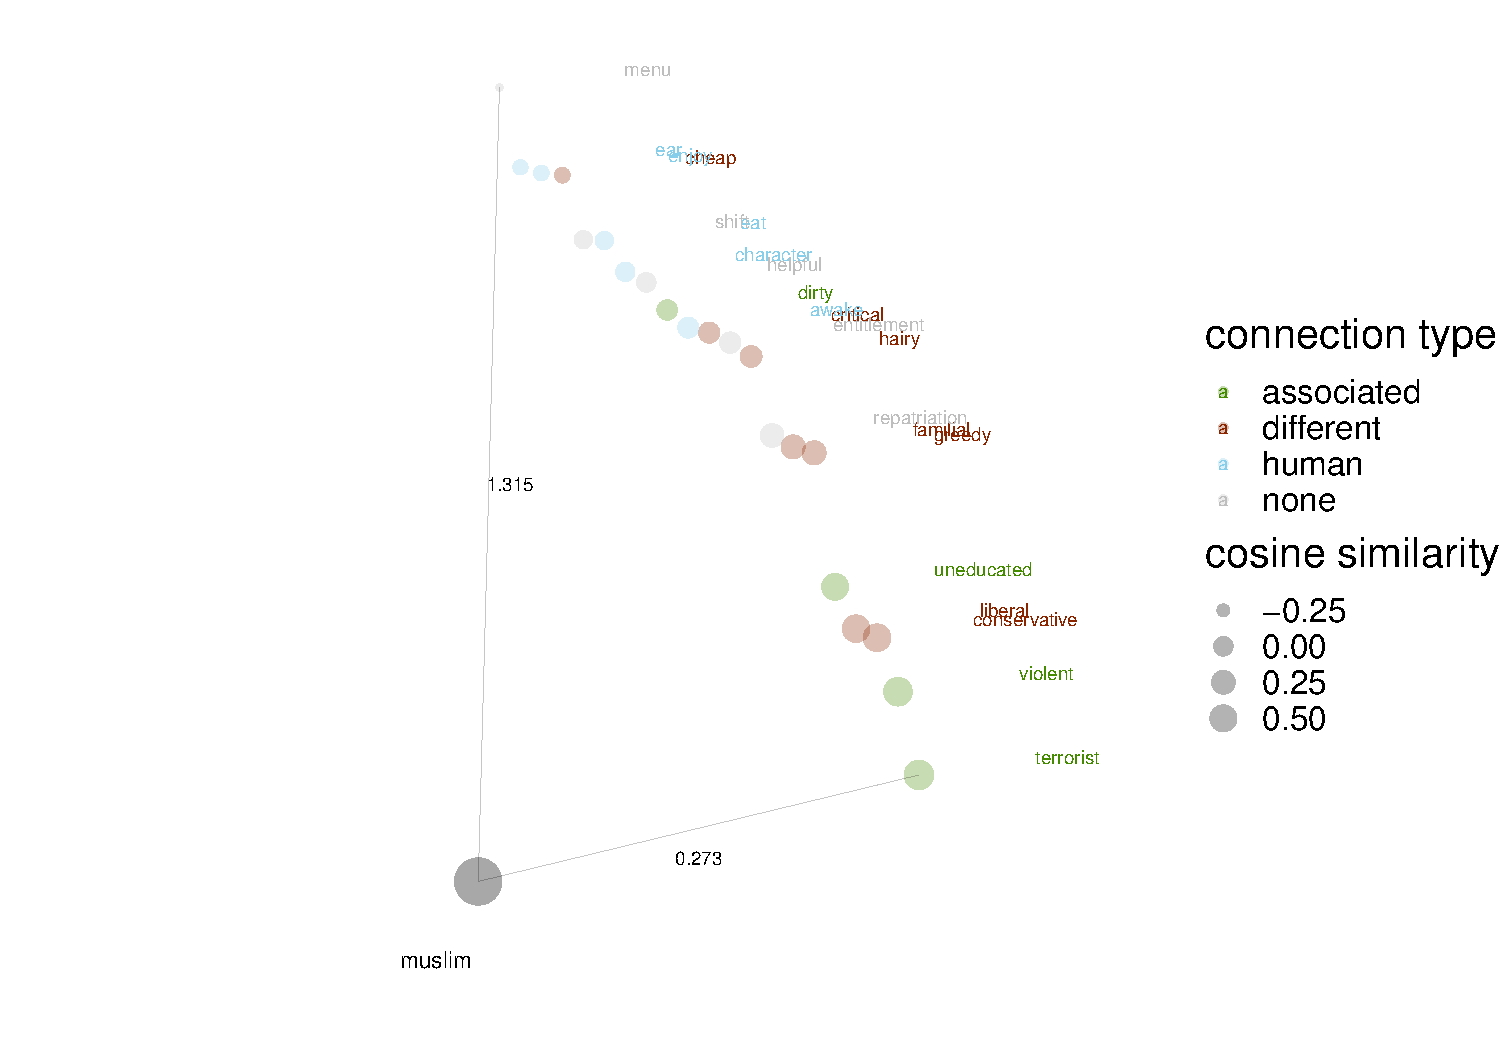
\includegraphics[width=0.7\linewidth]{presentationESSLLI_files/figure-beamer/unnamed-chunk-4-1} \end{center}
\end{center}

Then \(\pr(H \vert E) =[0,1]\), no matter what the evidence says.

\vspace{1mm} \scriptsize

({\textbf{???}},({\textbf{???}}), {\textbf{???}}, {\textbf{???}},
{\textbf{???}}, {\textbf{???}})

\end{block}

\end{frame}

\begin{frame}{Epistemological challenges}

\begin{block}{Mystery coins}

\begin{itemize}
\tightlist
\item
  A fair draw of one of two biased coins, with biases \(.4, and .6\).
\end{itemize}

\pause

\vspace{-2mm}

\begin{itemize}
\tightlist
\item
  Imprecise reaction: \(\{.4, .6\}\).
\end{itemize}

\pause

\vspace{-2mm}

\begin{itemize}
\tightlist
\item
  Precise probabilism: expected bias of \(.5\).
\end{itemize}

\pause

\end{block}

\begin{block}{Question}

As far as accuracy is concerned, why prefer the imprecise way?

Say the actual bias is .4. A first stab:

\vspace{-3mm}

\begin{align*}
\mathsf{inaccuracy(imprecise)} & = \frac{0 + .2}{2} = .1\\
\mathsf{inaccuracy(precise)} & =  .1\\
\end{align*}

\vspace{-5mm} \scriptsize

({\textbf{???}}, {\textbf{???}}; Schoenfield,
\protect\hyperlink{ref-schoenfield2017AccuracyRationalityImprecise}{2017})

\end{block}

\end{frame}

\begin{frame}{Higher-order approach}

\begin{block}{The mystery coin with \((.2,.8)\) and 1 head in five
tosses}

\begin{center}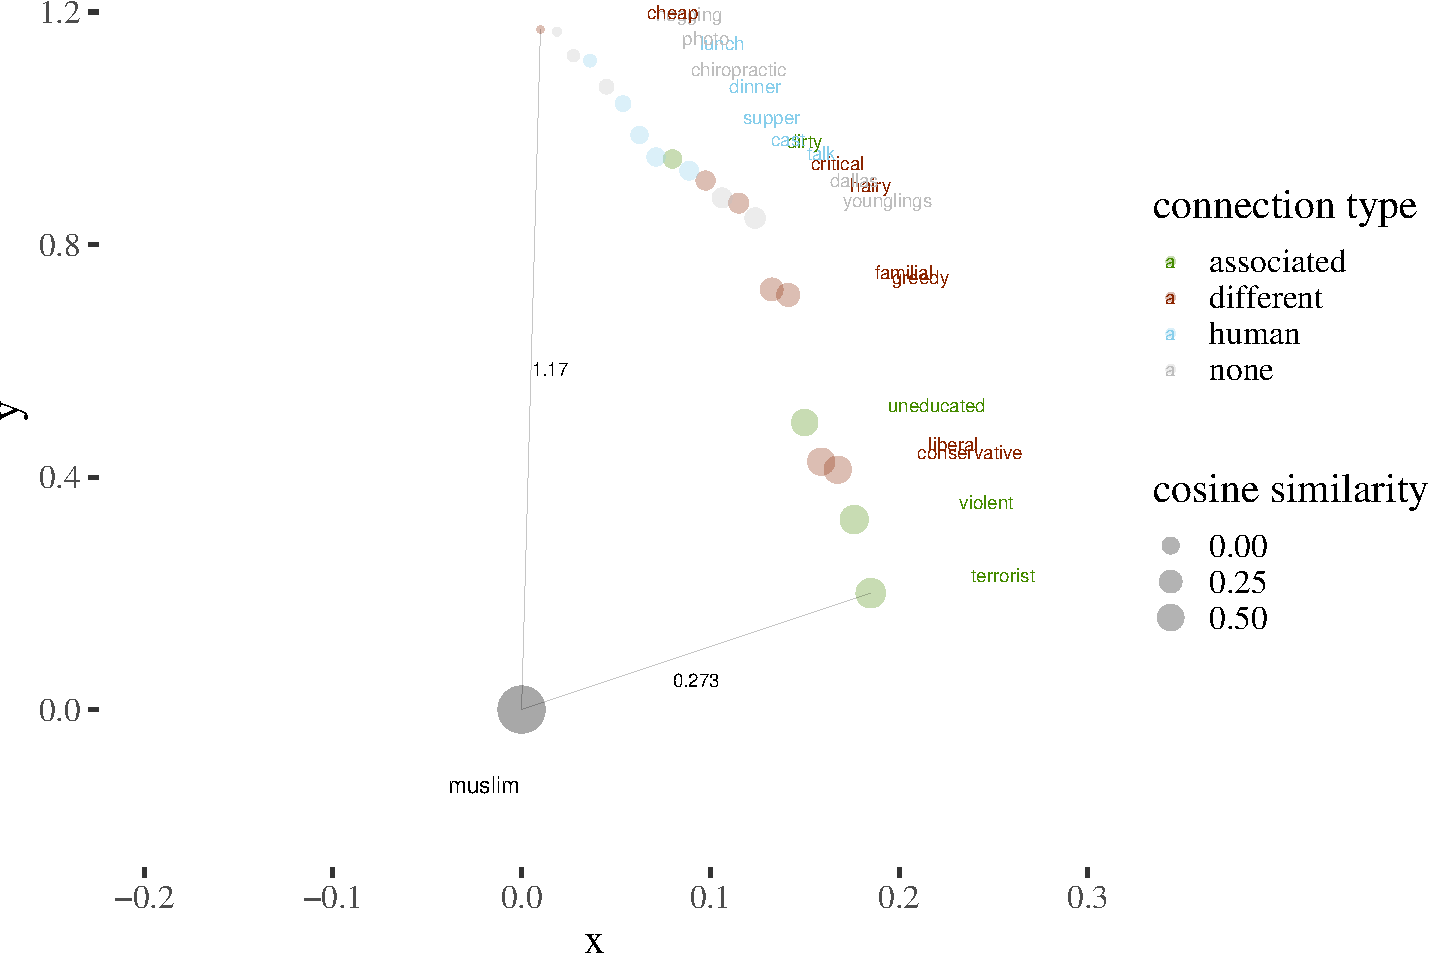
\includegraphics[width=0.9\linewidth]{presentationESSLLI_files/figure-beamer/unnamed-chunk-5-1} \end{center}

\end{block}

\end{frame}

\begin{frame}{Higher-order approach}

\begin{block}{Two experts, uniform prior}

\begin{center}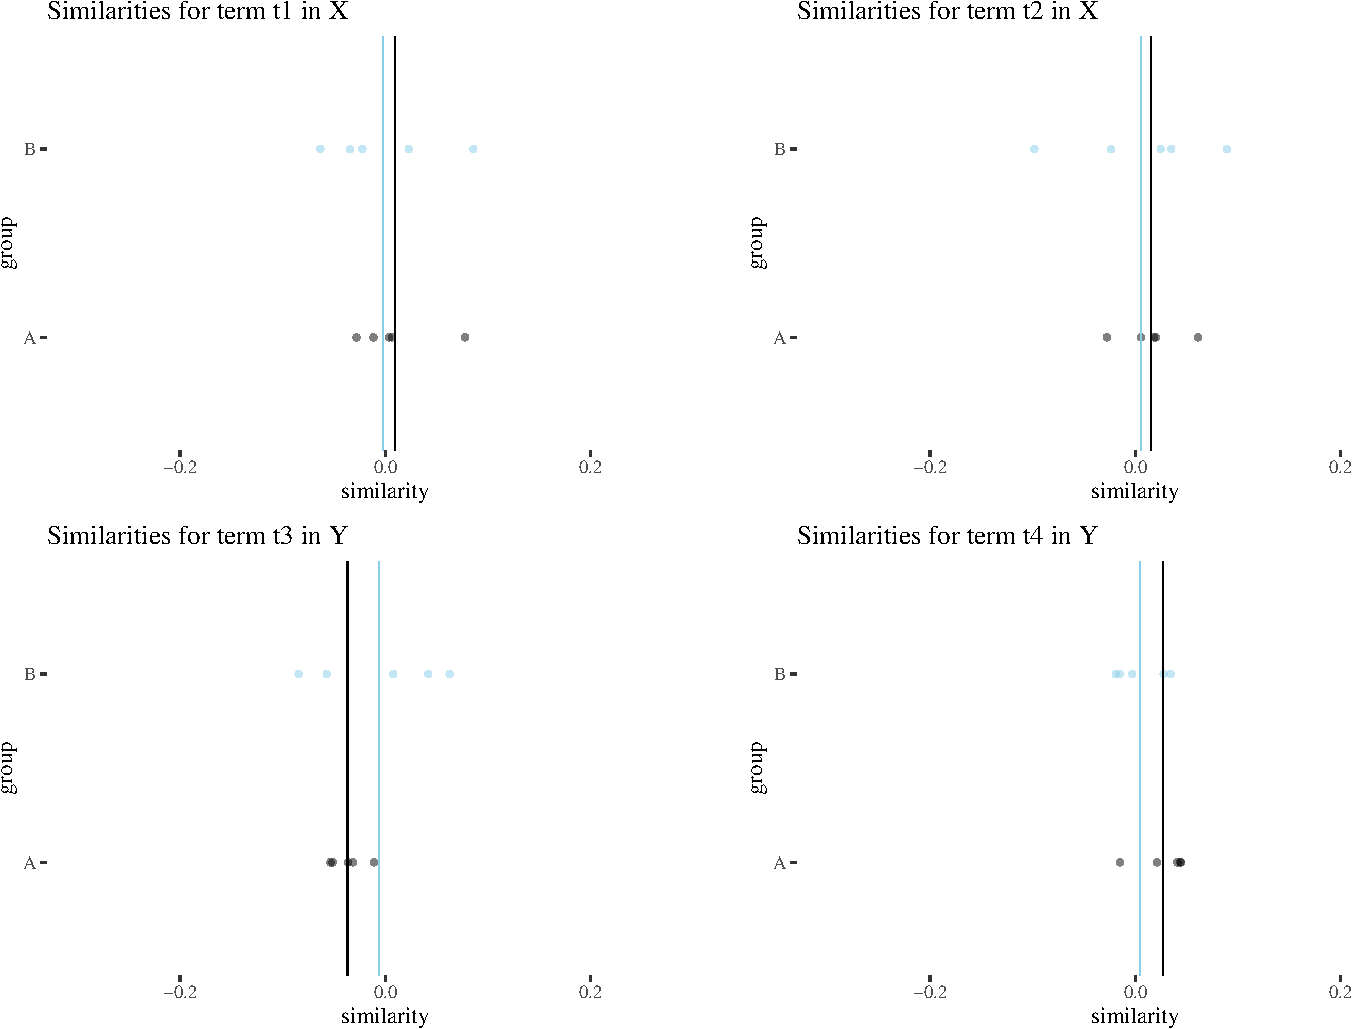
\includegraphics[width=0.9\linewidth]{presentationESSLLI_files/figure-beamer/unnamed-chunk-6-1} \end{center}

\end{block}

\end{frame}

\begin{frame}{The key conjecture}

\begin{block}{With higher-order methods, it will be possible to:}

\begin{itemize}
\item
  match the representation of uncertainty with the evidence,
\item
  combine various sources of uncertainty without running into the known
  problems,
\item
  use existing mathematics to make sense of accuracy in such contexts,
\item
  capture reasoning with radical uncertainty without dilation and belief
  inertia.
\end{itemize}

\end{block}

\end{frame}

\begin{frame}{Tasks (discussion)}

\footnotesize 

\begin{itemize}
\tightlist
\item
  Relate this representation to weight of evidence.
\end{itemize}

\vspace{-2mm}

\begin{itemize}
\item
  Go beyond grid approximation and beta representation.
\item
  Represent agnosticism so that:

  \begin{itemize}
  \item
    agnosticism preservation holds, and
  \item
    inertia fails.
  \end{itemize}
\end{itemize}

\vspace{-2mm}

\begin{itemize}
\tightlist
\item
  Represent opinion aggregation more generally, compare to known
  limitations and features of already studied opinion pooling methods.
\end{itemize}

\vspace{-2mm}

\begin{itemize}
\tightlist
\item
  Investigate dilation-like phenomena in this context.
\end{itemize}

\vspace{-2mm}

\begin{itemize}
\tightlist
\item
  Study known distance functions between probabilistic measures as
  candidates for key elements of accuracy measures.
\end{itemize}

\vspace{-2mm}

\begin{itemize}
\tightlist
\item
  Explain away the apparent contrast between evidence-grounding and
  accuracy considerations (Easwaran \& Fitelson,
  \protect\hyperlink{ref-easwaranAndFitelson2015}{2015}).
\end{itemize}

\begin{center}
\Large Thank you for your attention!
\end{center}

\end{frame}

\begin{frame}{References}

\tiny

\hypertarget{refs}{}
\hypertarget{ref-easwaranAndFitelson2015}{}
Easwaran, K., \& Fitelson, B. (2015). Accuracy, coherence, and evidence.
In T. S. Gendler \& J. Hawthorne (Eds.), \emph{Oxford studies in
epistemology} (Vol. 5). Oxford University Press.

\hypertarget{ref-schoenfield2017AccuracyRationalityImprecise}{}
Schoenfield, M. (2017). The Accuracy and Rationality of Imprecise
Credences: The Accuracy and Rationality of Imprecise Credences.
\emph{Noûs}, \emph{51}(4), 667--685.
\url{https://doi.org/10.1111/nous.12105}

\hypertarget{ref-walley1991statistical}{}
Walley, P. (1991). \emph{Statistical reasoning with imprecise
probabilities}. Chapman; Hall London.

\end{frame}

\end{document}
